\section{Cooling and Interlocks}
\label{sec:proc_cooling}
\subsection{Start FEB chiller}
\begin{enumerate}
    \item Disable the FEB flow interlock.
    \item Verify that the temperature setpoint is 20 C. If not, call the SVT expert.
    \item Check the RTD temperature limits. The low limits should be set at 15 C and the high limits at 25 C. If not, call the SVT expert.
    \item Verify that all PLC alarms that affect the FEB chiller loop (supply RTD, return RTD, and vacuum) are in ``Ok'' state.
    \item Verify that the FEB valve is open.
    \item Start the chiller.
    \item Wait for the flow switch value to change, then enable the FEB flow interlock.
        If the flow switch does not trigger, call the SVT expert.
    \item At this point, the FEBs can be powered.
    \item The \textbf{current temperature} shown in the FEB chiller GUI should converge to the setpoint in a few minutes.
    \item When the temperature has reached the setpoint, lower the high limits in the interlock to their final values.
\end{enumerate}

\subsection{Start SVT chiller}
\begin{enumerate}
    \item Change the chiller temperature setpoint to 20 C. (This assumes the SVT cooling loop is at room temperature to start. If it is cold, call the SVT expert for permission to use a lower starting setpoint.)
    \item Check the RTD temperature limits in the PLC GUI. The low limits should be set at their final values. Change the high limits to 25 C.
    \item Verify that of the PLC alarms that affect the SVT chiller loop (flow, supply RTD, return RTD, and vacuum), the first (flow) is in ``Fault'' state, and the rest are in ``Ok'' state.
    \item Verify that of the software interlocks that affect the SVT chiller loop (supply RTD, return RTD, and vacuum), all are in ``Ok'' state.
    \item Disable the SVT flow interlock.
        Now all PLC alarms and software interlocks should be in ``Ok'' state, and the SVT valve should be open.
        If not, call the SVT expert.
    \item Start the chiller.
    \item Wait for the flow switch value to change, then enable the SVT flow interlock.
        If the flow switch does not change, call the SVT expert.
    \item Wait for the chiller temperature to stabilize at the setpoint.
        Some oscillation is normal in the short term, and the chiller may trip off (most likely if the chiller has been off for a while).
        If this happens, call the SVT expert to have the chiller reset, and start over from the beginning of the procedure.
    \item Lower the chiller temperature setpoint by 10 C (to 10 C).
        Wait 20 minutes for temperatures to equalize in the system (chiller temperature and RTDs should stabilize in about 10 minutes). If at the end of this time the chiller temperature is more than 0.5 C away from setpoint, or either RTD is more than 3 C away from setpoint, call the SVT expert.
    \item Repeat the previous step (lower setpoint by 10 C, wait for 20 minutes)  until the setpoint reaches its final value.
    \item After the final waiting period, change the high limits in the PLC GUI to their final values.
\end{enumerate}

\subsection{Stop FEB chiller}
\begin{enumerate}
    \item Verify that hybrid bias, FEB power, and flange board power are off.
    \item Press the \textbf{Stop} button in the FEB chiller GUI. The interlocks will close the FEB valve and trip the MPOD.
\end{enumerate}

\subsection{Stop SVT chiller}
\begin{enumerate}
    \item Verify that hybrid bias, FEB power, and flange board power are off.
    \item Press the \textbf{Stop} button in the SVT chiller GUI. The interlocks will close the SVT valve and trip the MPOD.
\end{enumerate}

\subsection{Draining SVT chiller (experts only)}
\begin{enumerate}
    \item Disable the PLC interlocks for flow, supply RTD, and return RTD.
    \item Put the chiller in manual mode using the touchscreen.
    \item Follow the instructions in the chiller manual to drain the chiller. Use the big plastic jug and the two short pieces of rubber tube.

    \item When you disconnect a fitting in the chiller loop, drain both connections into a beaker.
    \item Purge both connections using the nitrogen line (use a Swagelok-to-VCR adapter with a used gasket), with the reservoir drain valve (the ball valve with a plastic handle) open.
        Be sure to cap the connection not being purged using a VCR cap and a used gasket. 
\end{enumerate}

\subsection{Filling SVT chiller from empty (experts only)}
\begin{enumerate}
    \item Disable the PLC interlocks for SVT chiller flow, supply RTD, and return RTD.
    \item Follow the instructions in the chiller manual to fill the chiller. Use the metal funnel.
    \item If the final level of the chiller is below 1/4, add a full jug of HFE 7000.
\end{enumerate}

\subsection{Changing SVT chiller temperature}
\label{sec:proc_svt_chiller_tempchange}
\begin{enumerate}
    \item Disable the PLC and software interlocks for SVT chiller supply RTD and return RTD (these are left disabled between run periods).
    \item Change the setpoint on the SVT chiller GUI in steps of no more than 10 degrees C.
        After each step, wait 20 minutes for temperatures to equalize in the system (chiller temperature and RTDs should stabilize in about 10 minutes).
        Check cooling lines for frost or melting ice.
    \item When at final temperature, change the alarm setpoints for the SVT chiller supply RTD and return RTD.
\end{enumerate}

\subsection{Adding fluid to SVT chiller}
\label{sec:proc_svt_chiller_refill}
The HFE-7000 fluid for the SVT cooling loop evaporates steadily and must be replenished approximately once every 3 weeks.
The fluid is supplied in 10-pound jugs. It is nontoxic and evaporates rapidly, so don't worry about small spills.
The chiller should be refilled when it reaches level 2 (slightly below 1/4); one jug will take it to level 7 (slightly above 3/4).
Refilling before the level drops to level 2 will cause a high level warning; waiting until the level drops to level 1 will cause a low level warning.

\begin{enumerate}
    \item Disable the PLC and software interlocks for SVT chiller supply RTD and return RTD (these are left disabled between run periods).
    \item Using a funnel, pour a jug of HFE-7000 into the fill port at the top of the chiller (open the metal cover and pull out the white plastic plug). If this causes a high level warning, acknowledge it.
    \item Once temperatures have stabilized, enable all interlocks that were bypassed.
    \item Check the water level in the FEB chiller.
    \item Make a logbook entry noting the chiller level before and after the fill, and the number of full HFE jugs remaining.
\end{enumerate}

\begin{figure}
    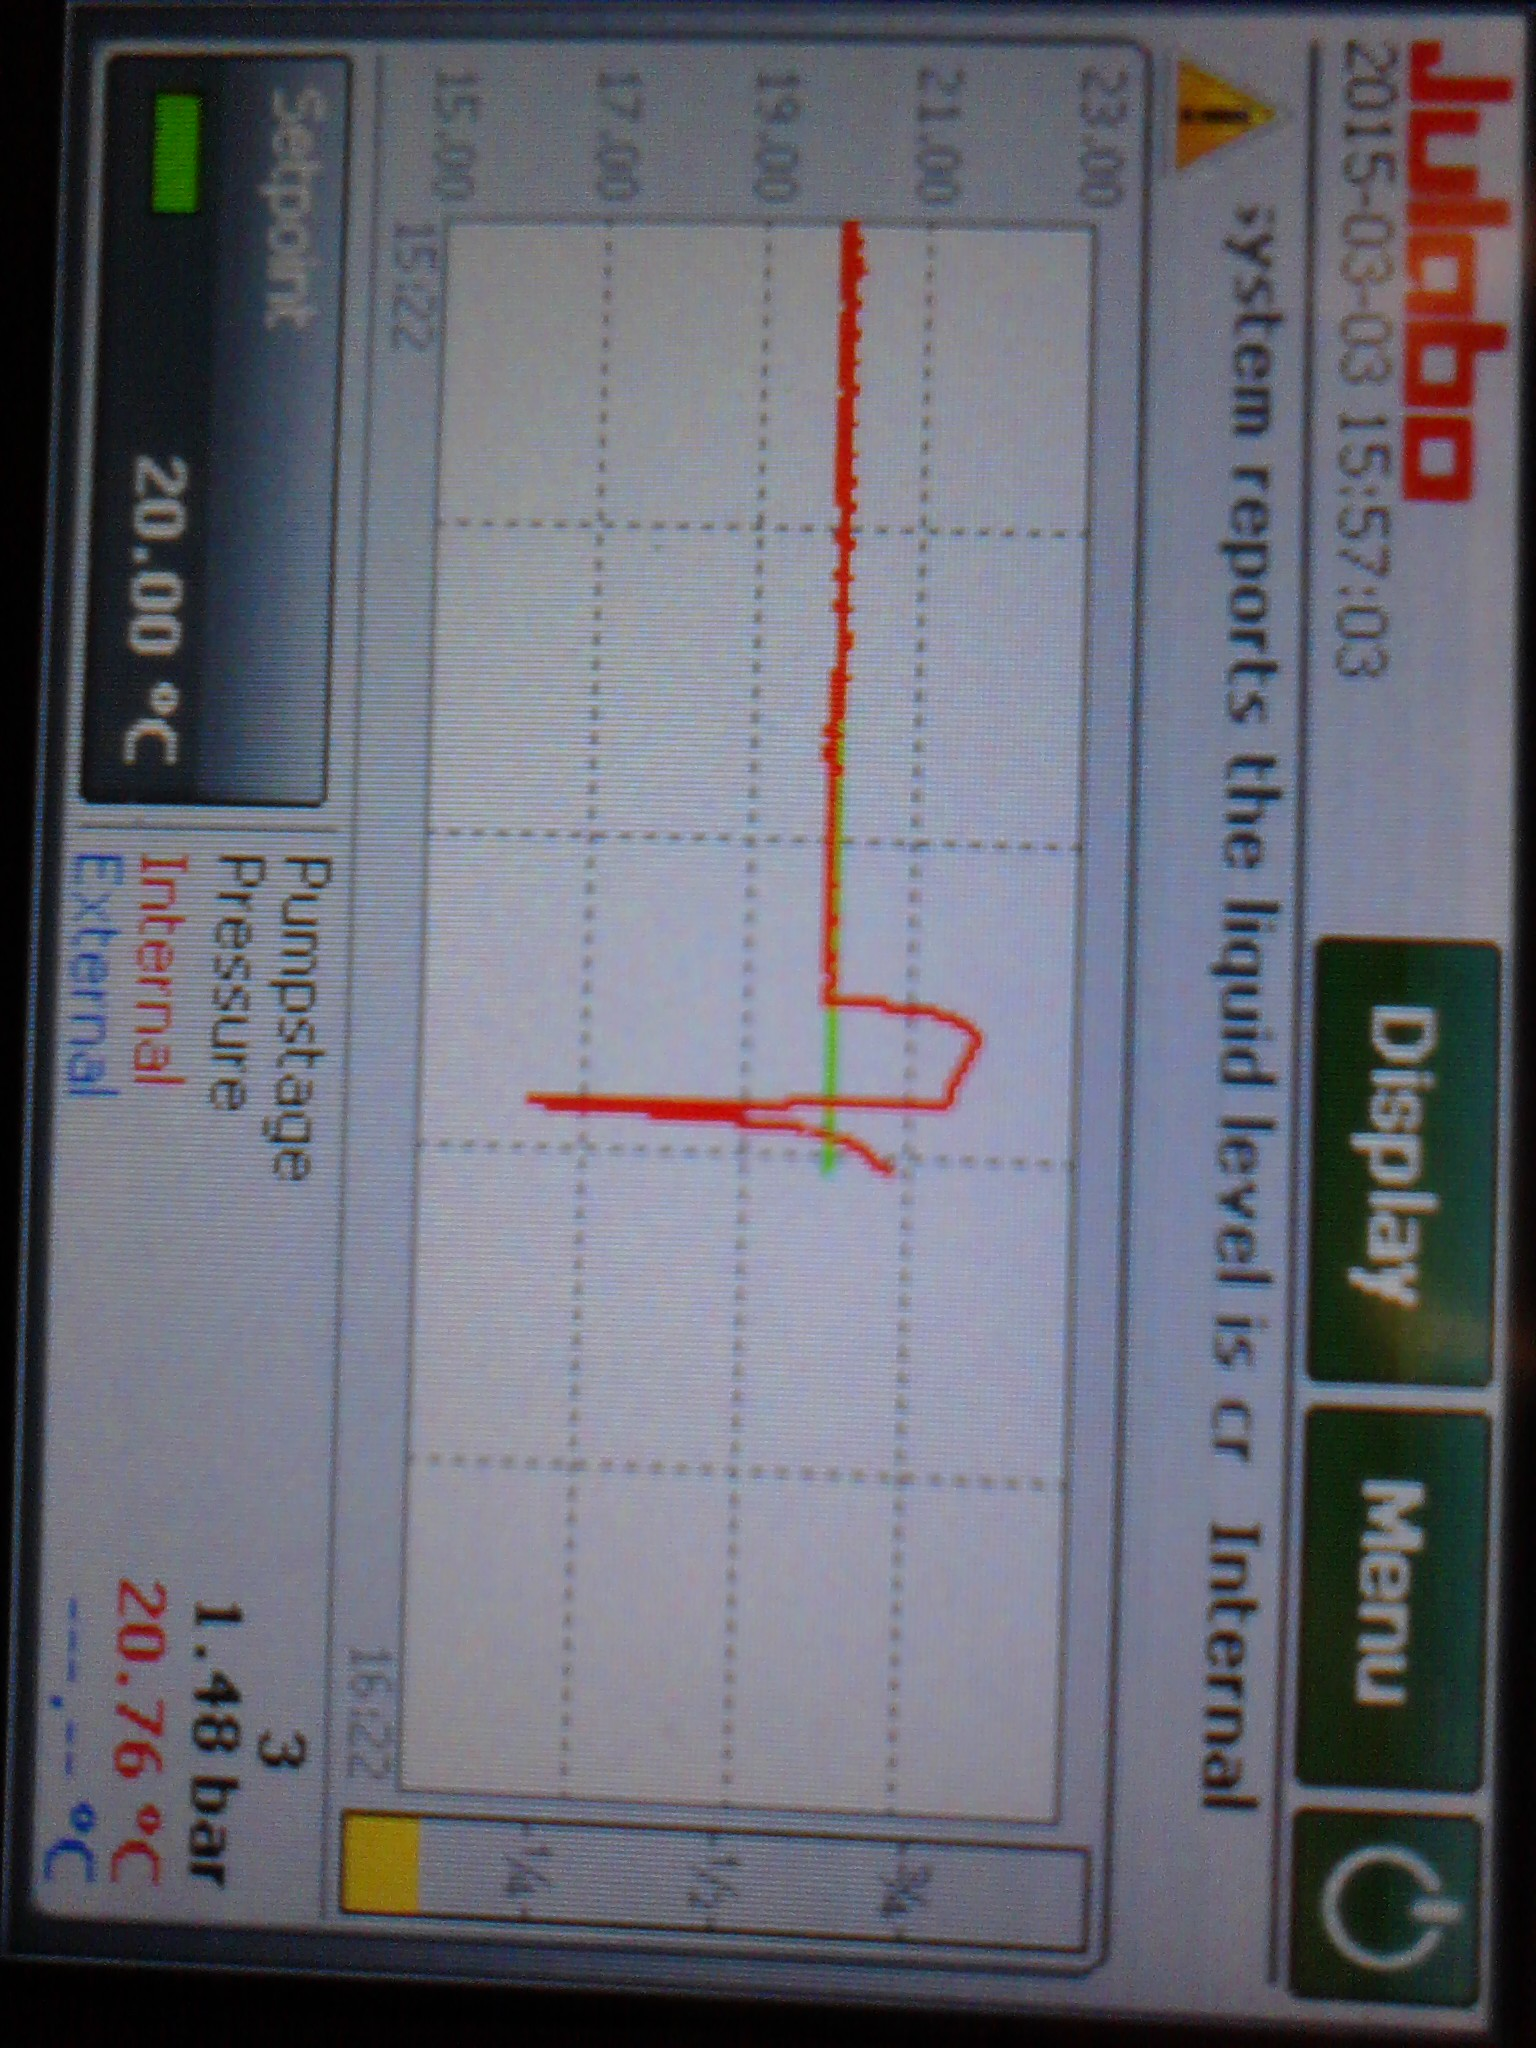
\includegraphics[angle=90,width=6cm]{figures/chiller_level1}
    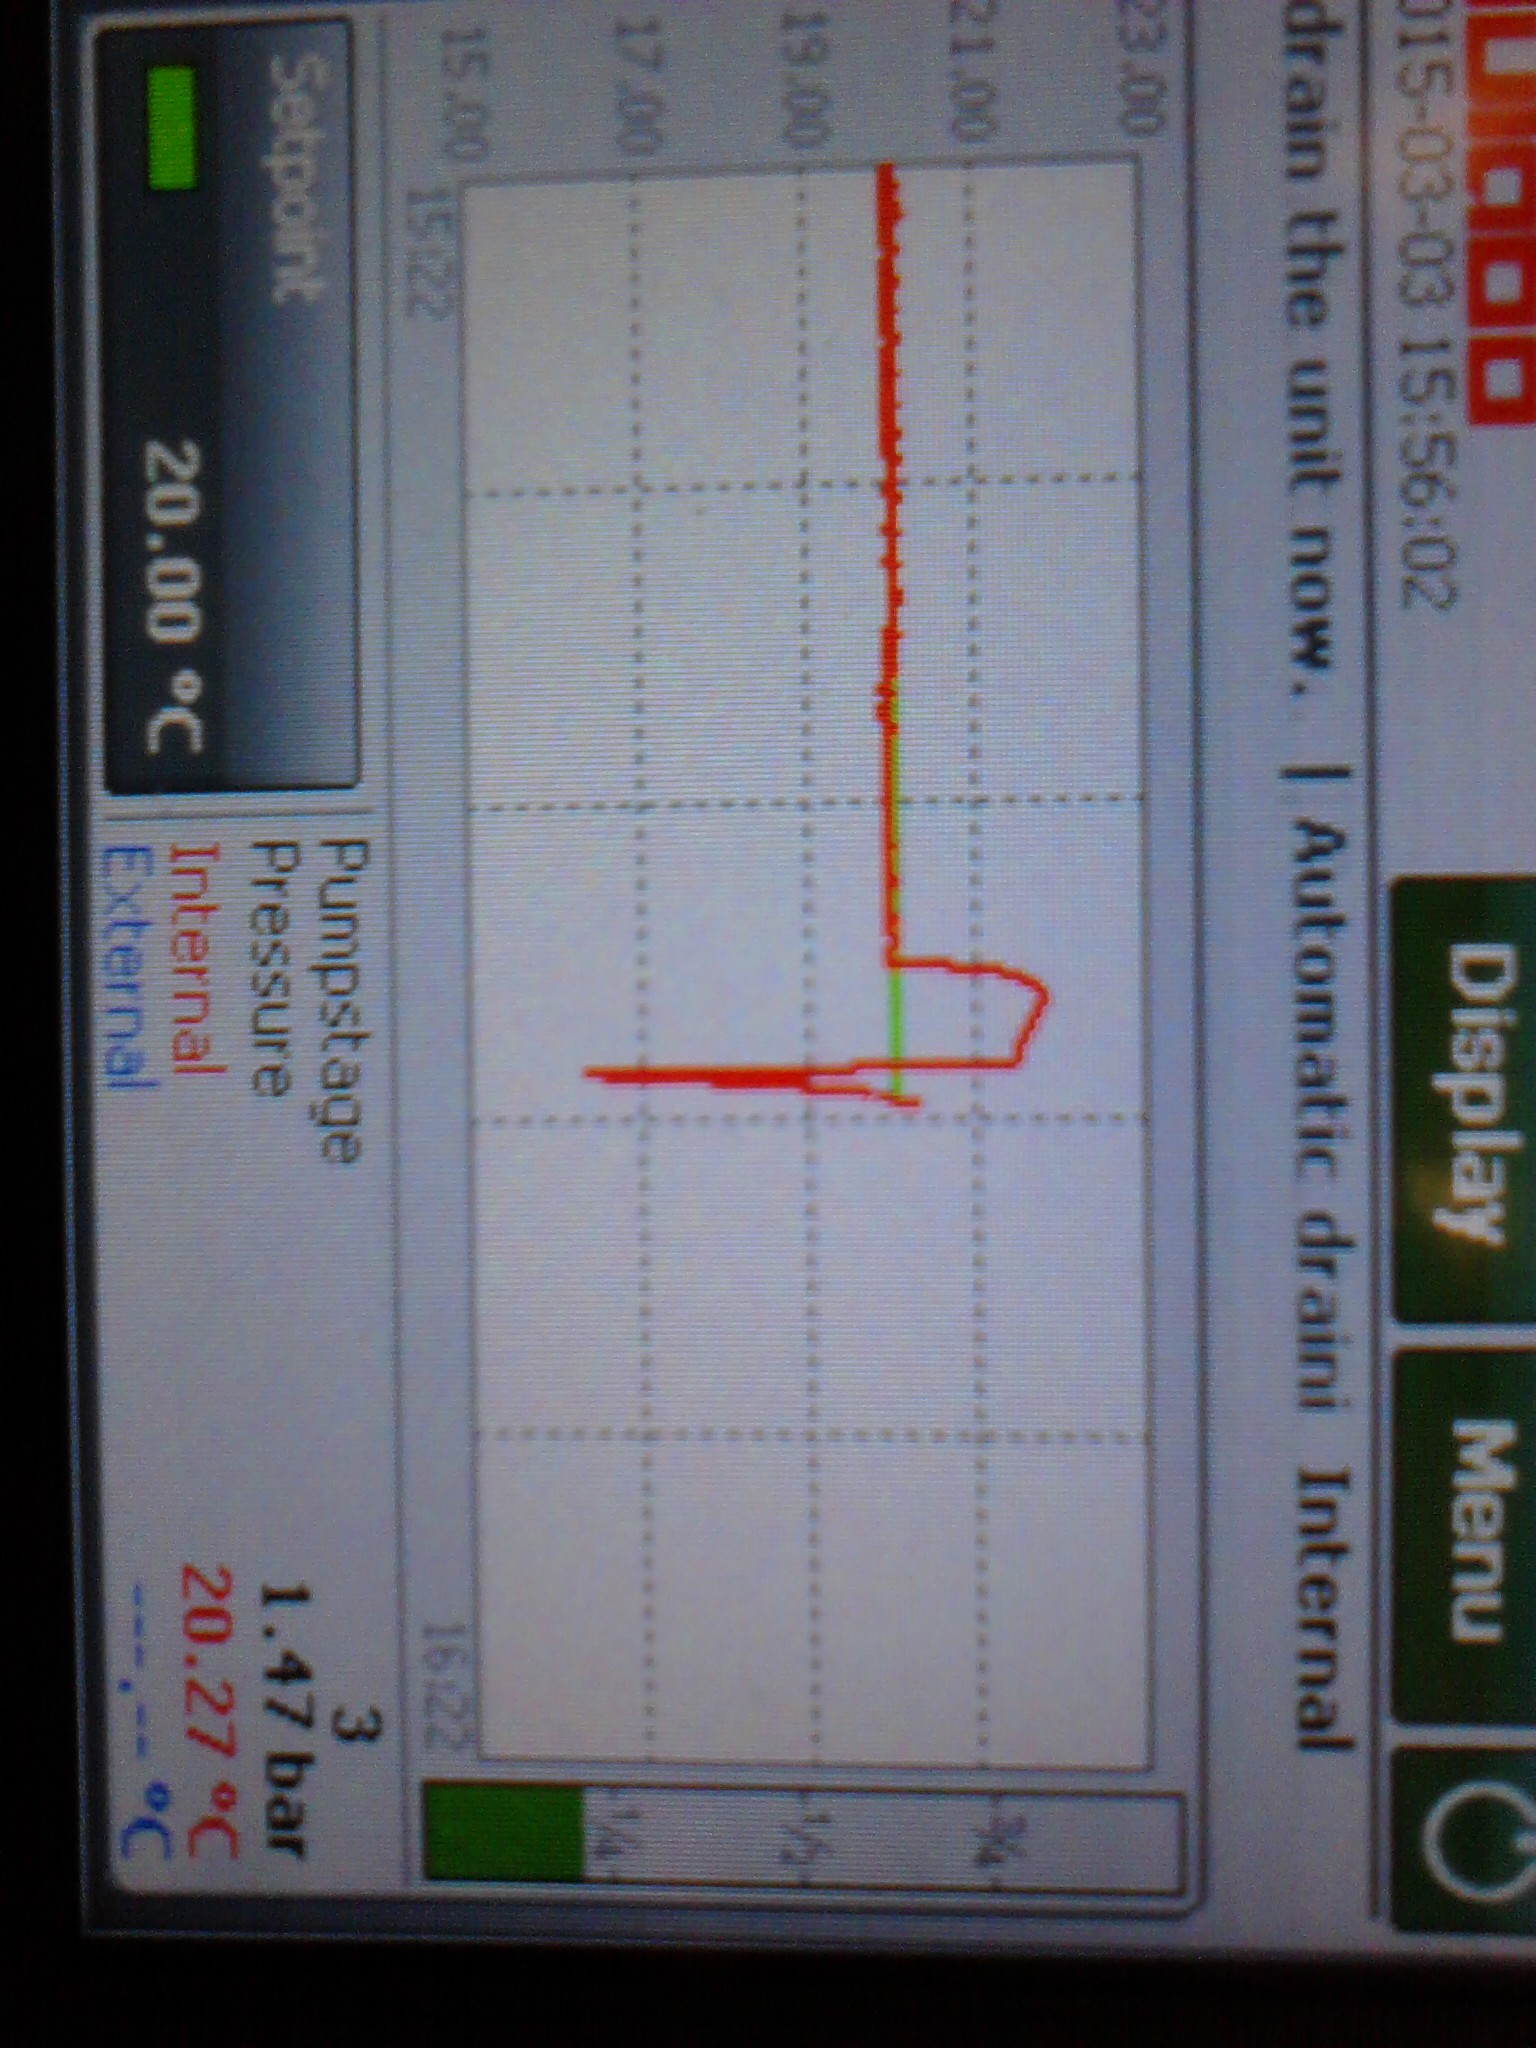
\includegraphics[angle=90,width=6cm]{figures/chiller_level2}
    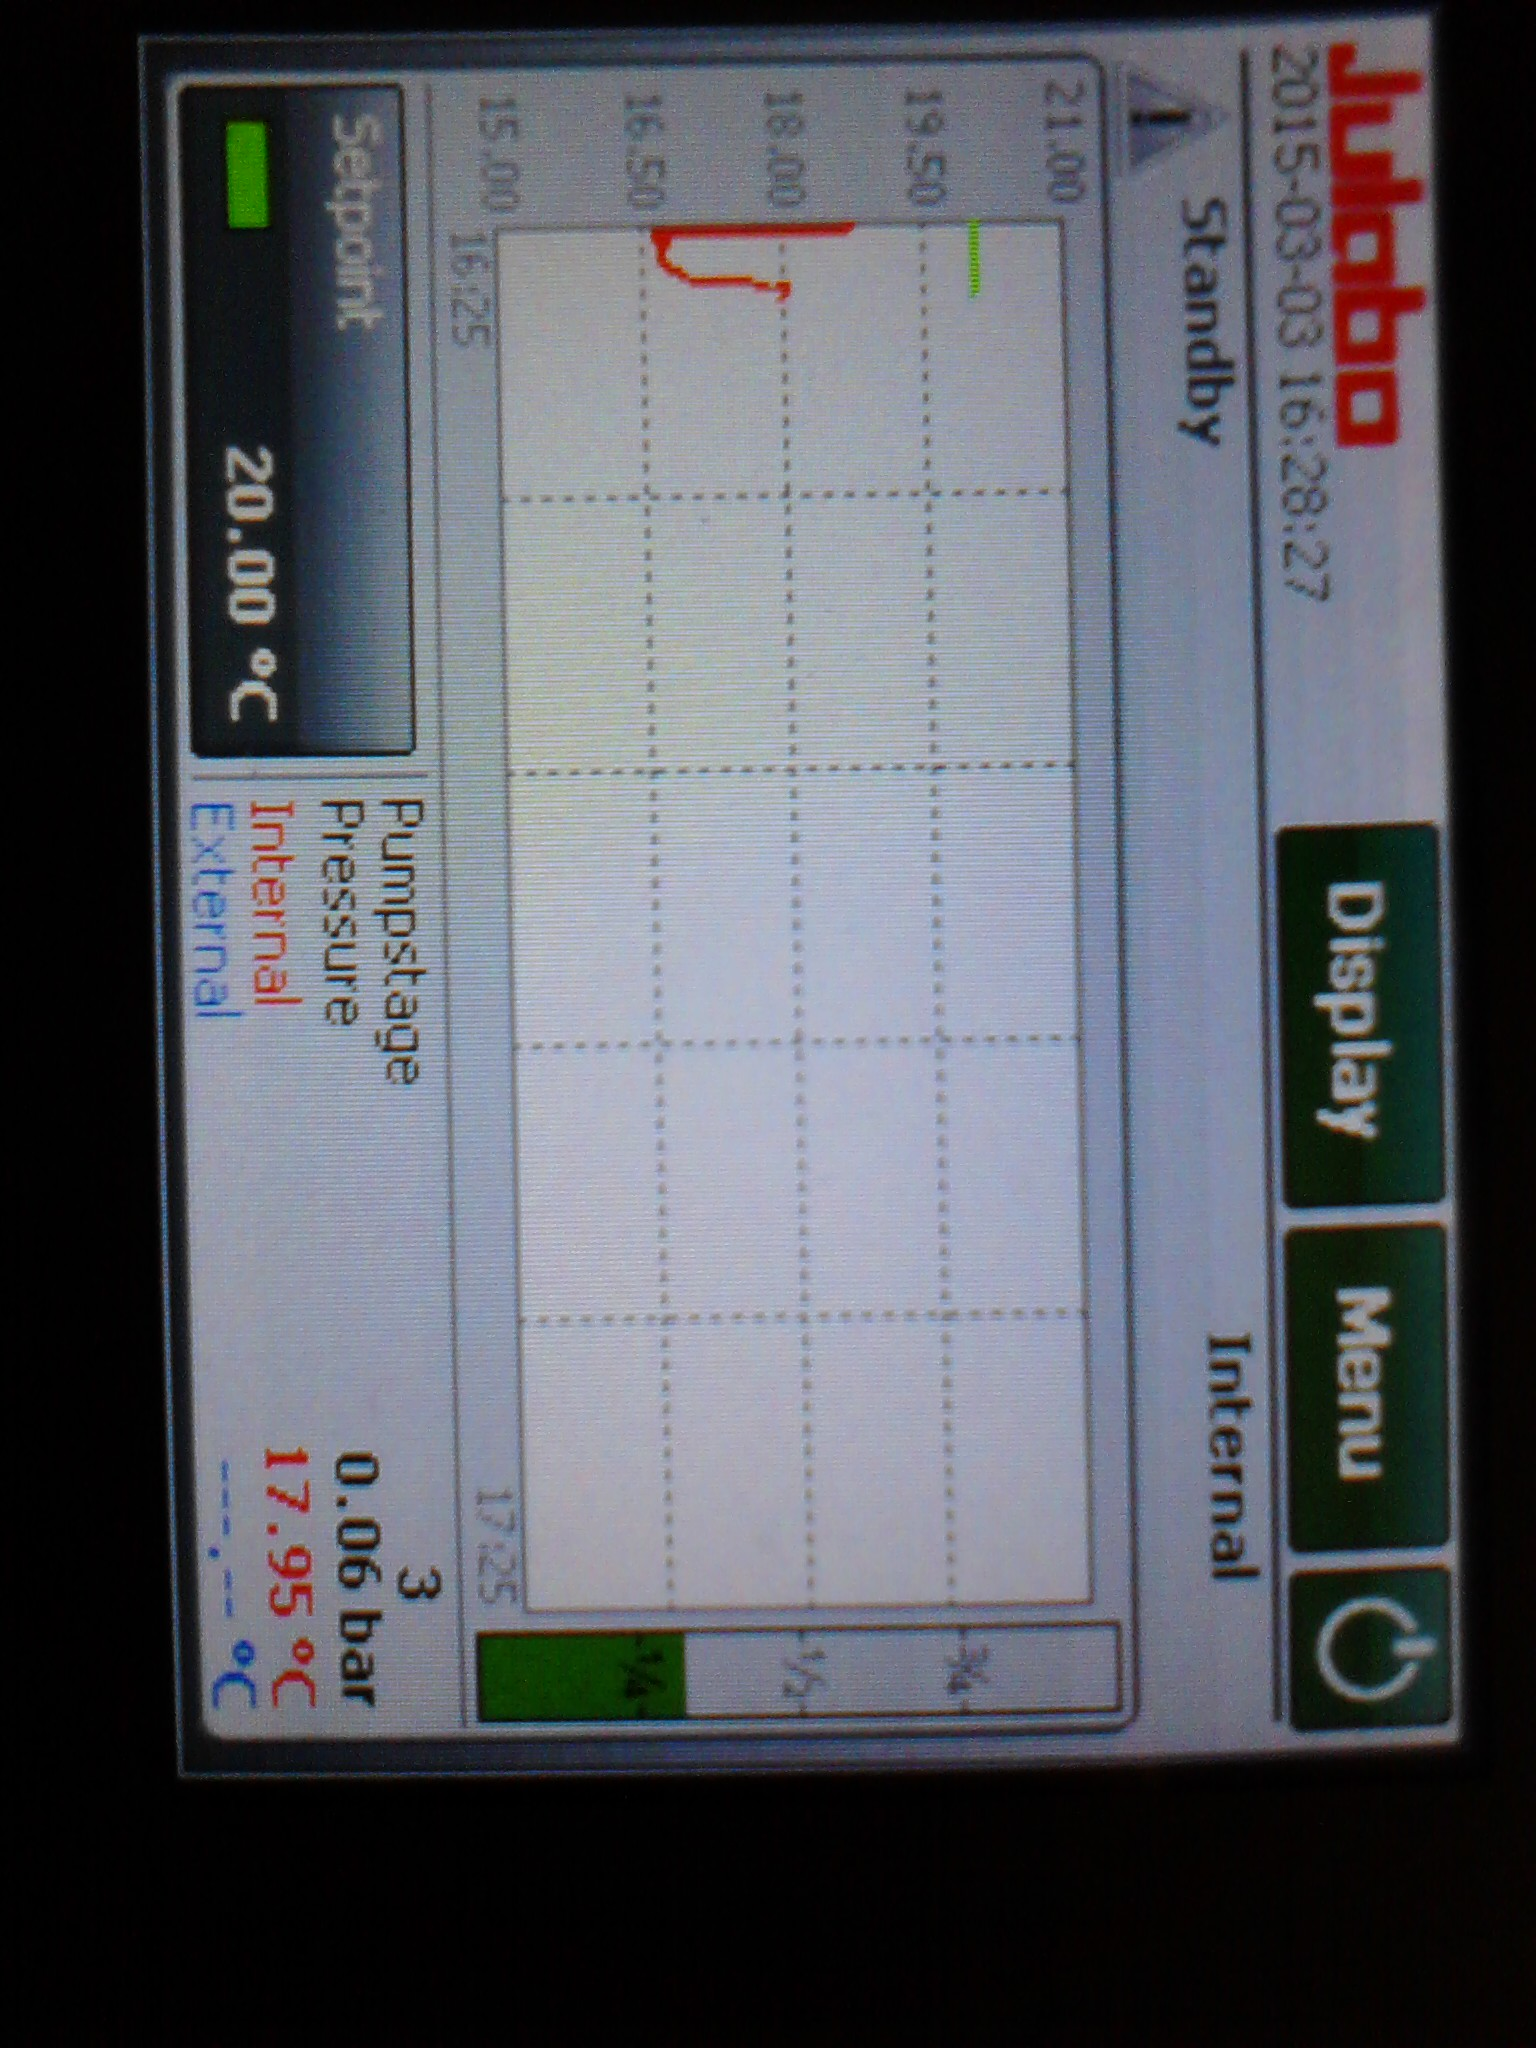
\includegraphics[angle=90,width=6cm]{figures/chiller_level3}
    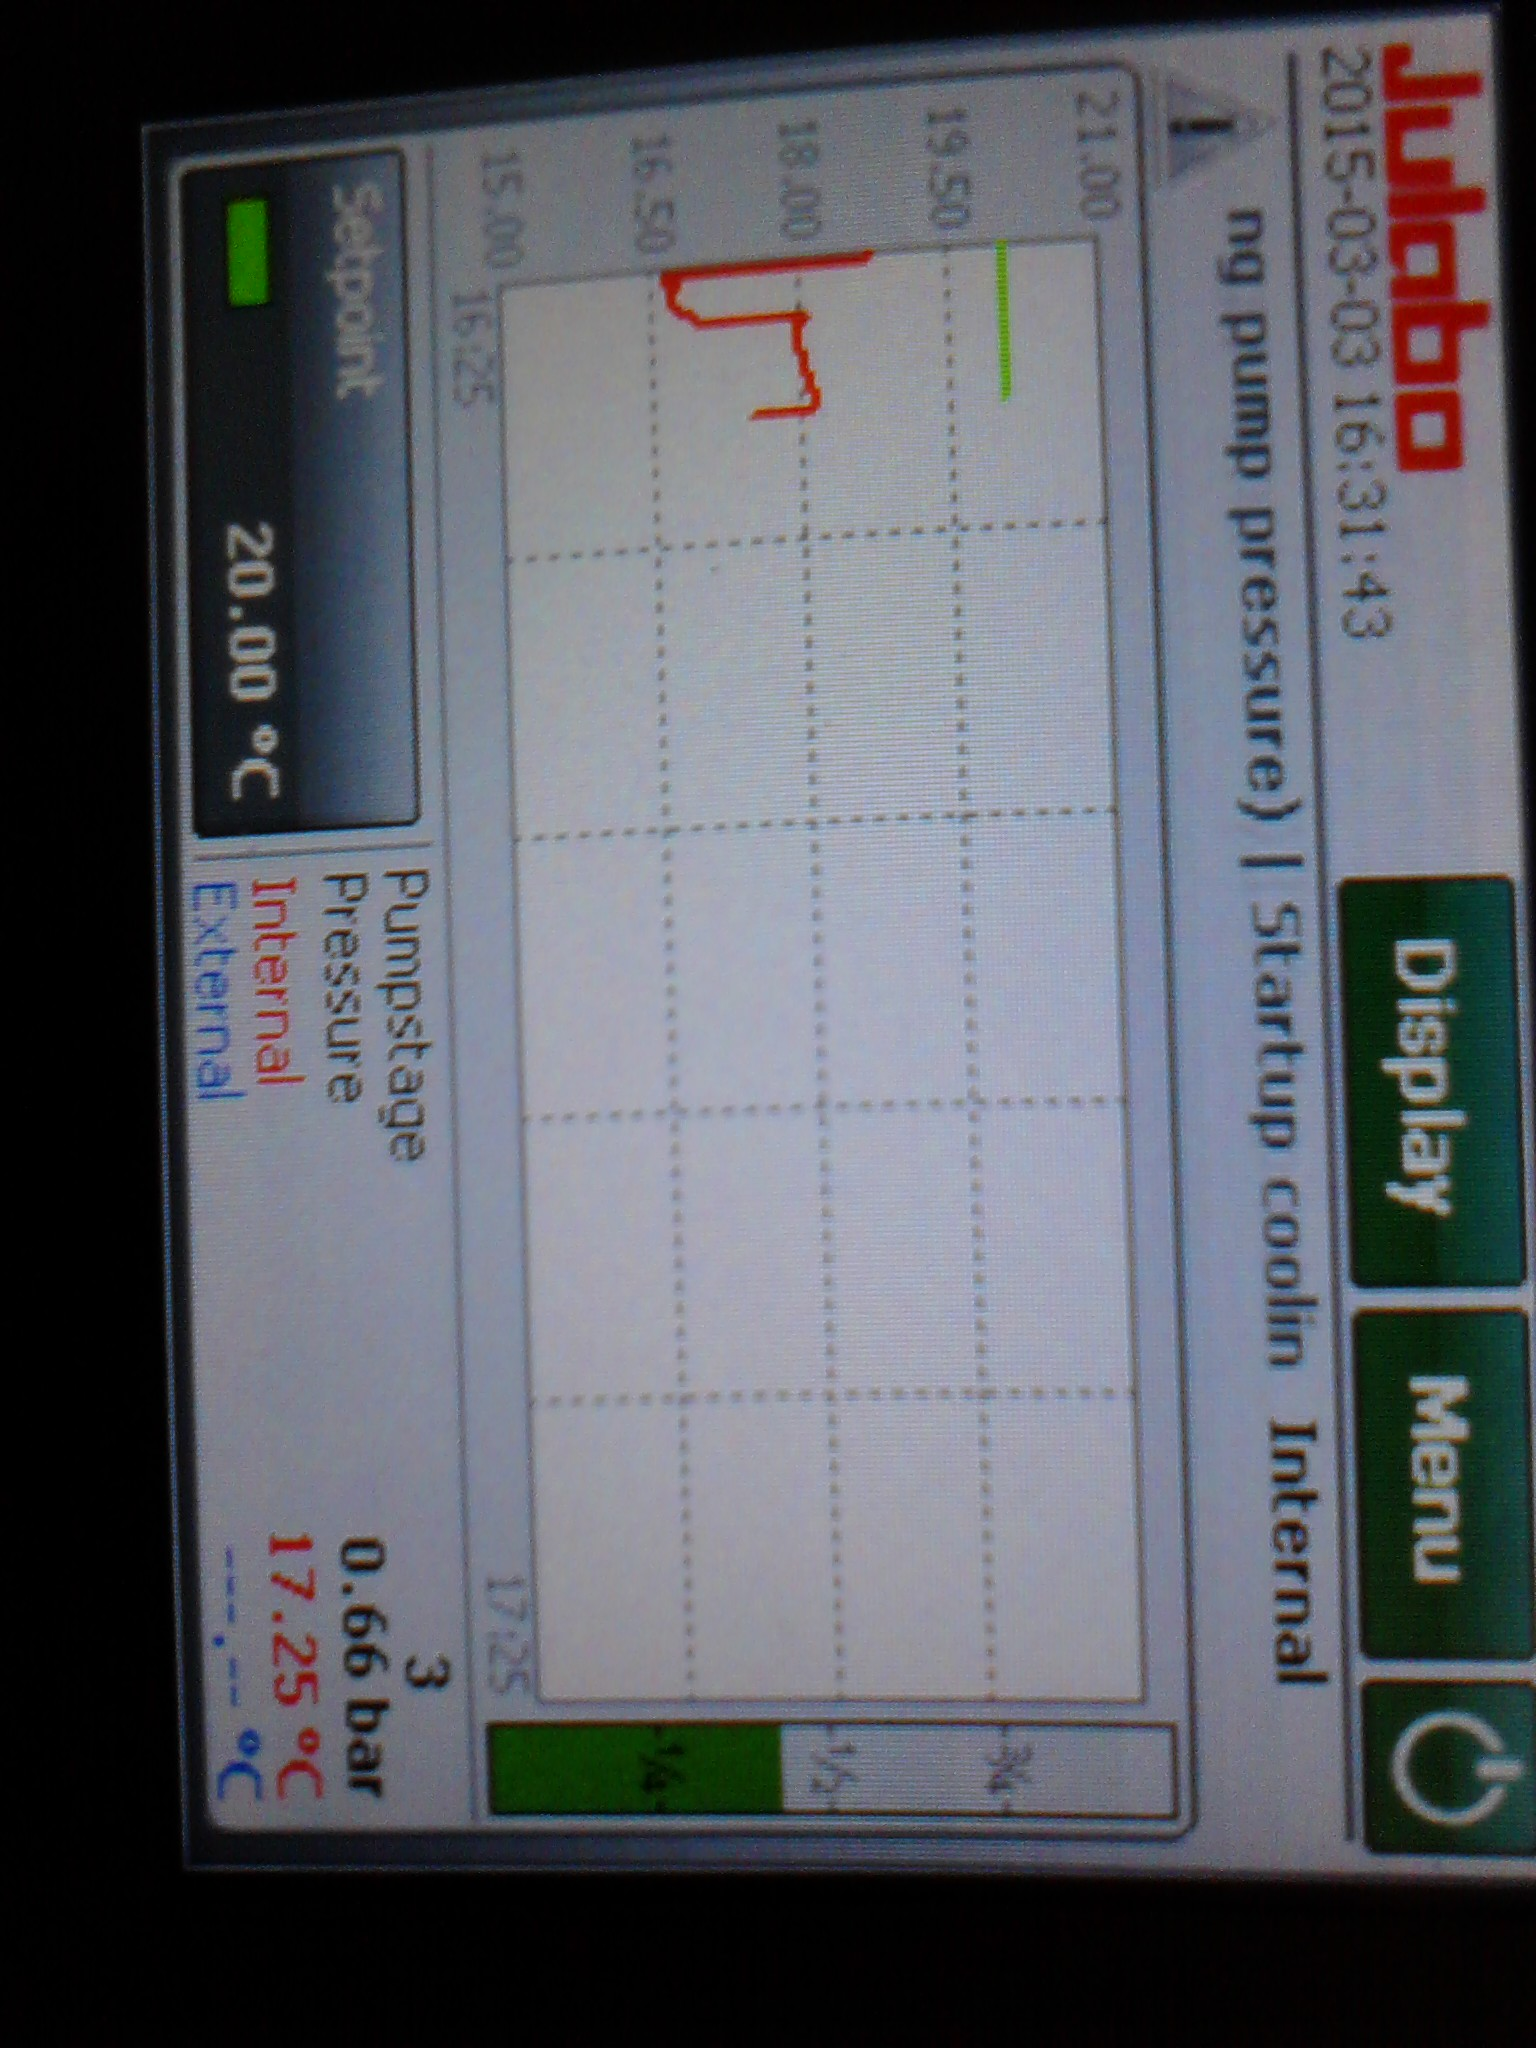
\includegraphics[angle=90,width=6cm]{figures/chiller_level4}
    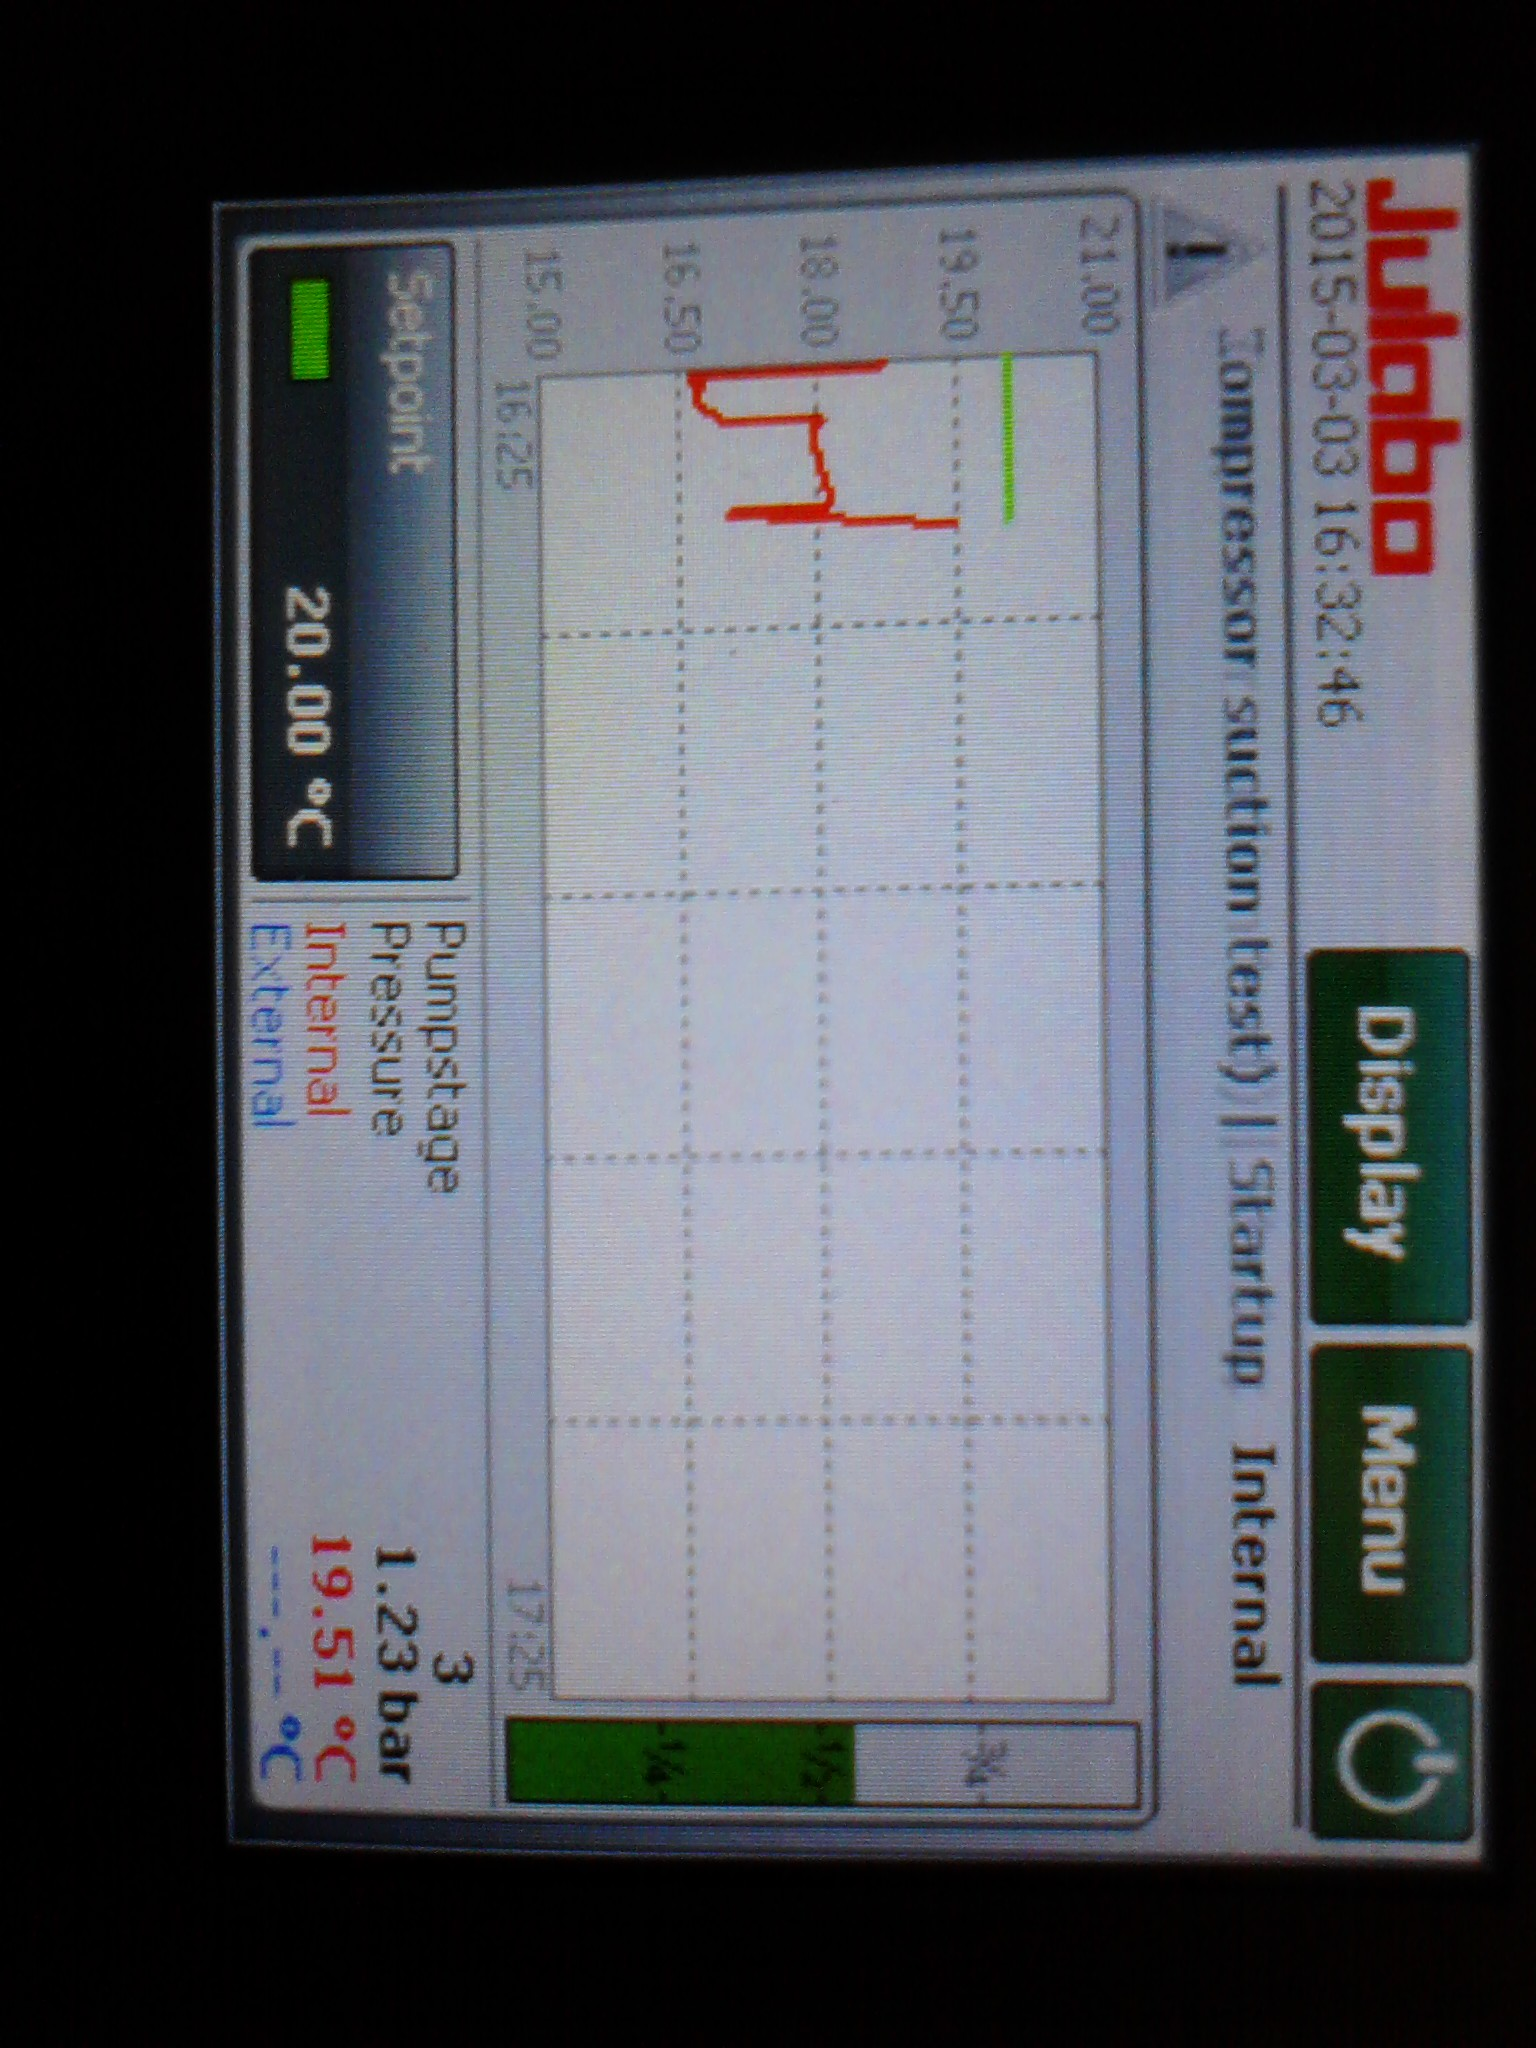
\includegraphics[angle=90,width=6cm]{figures/chiller_level5}
    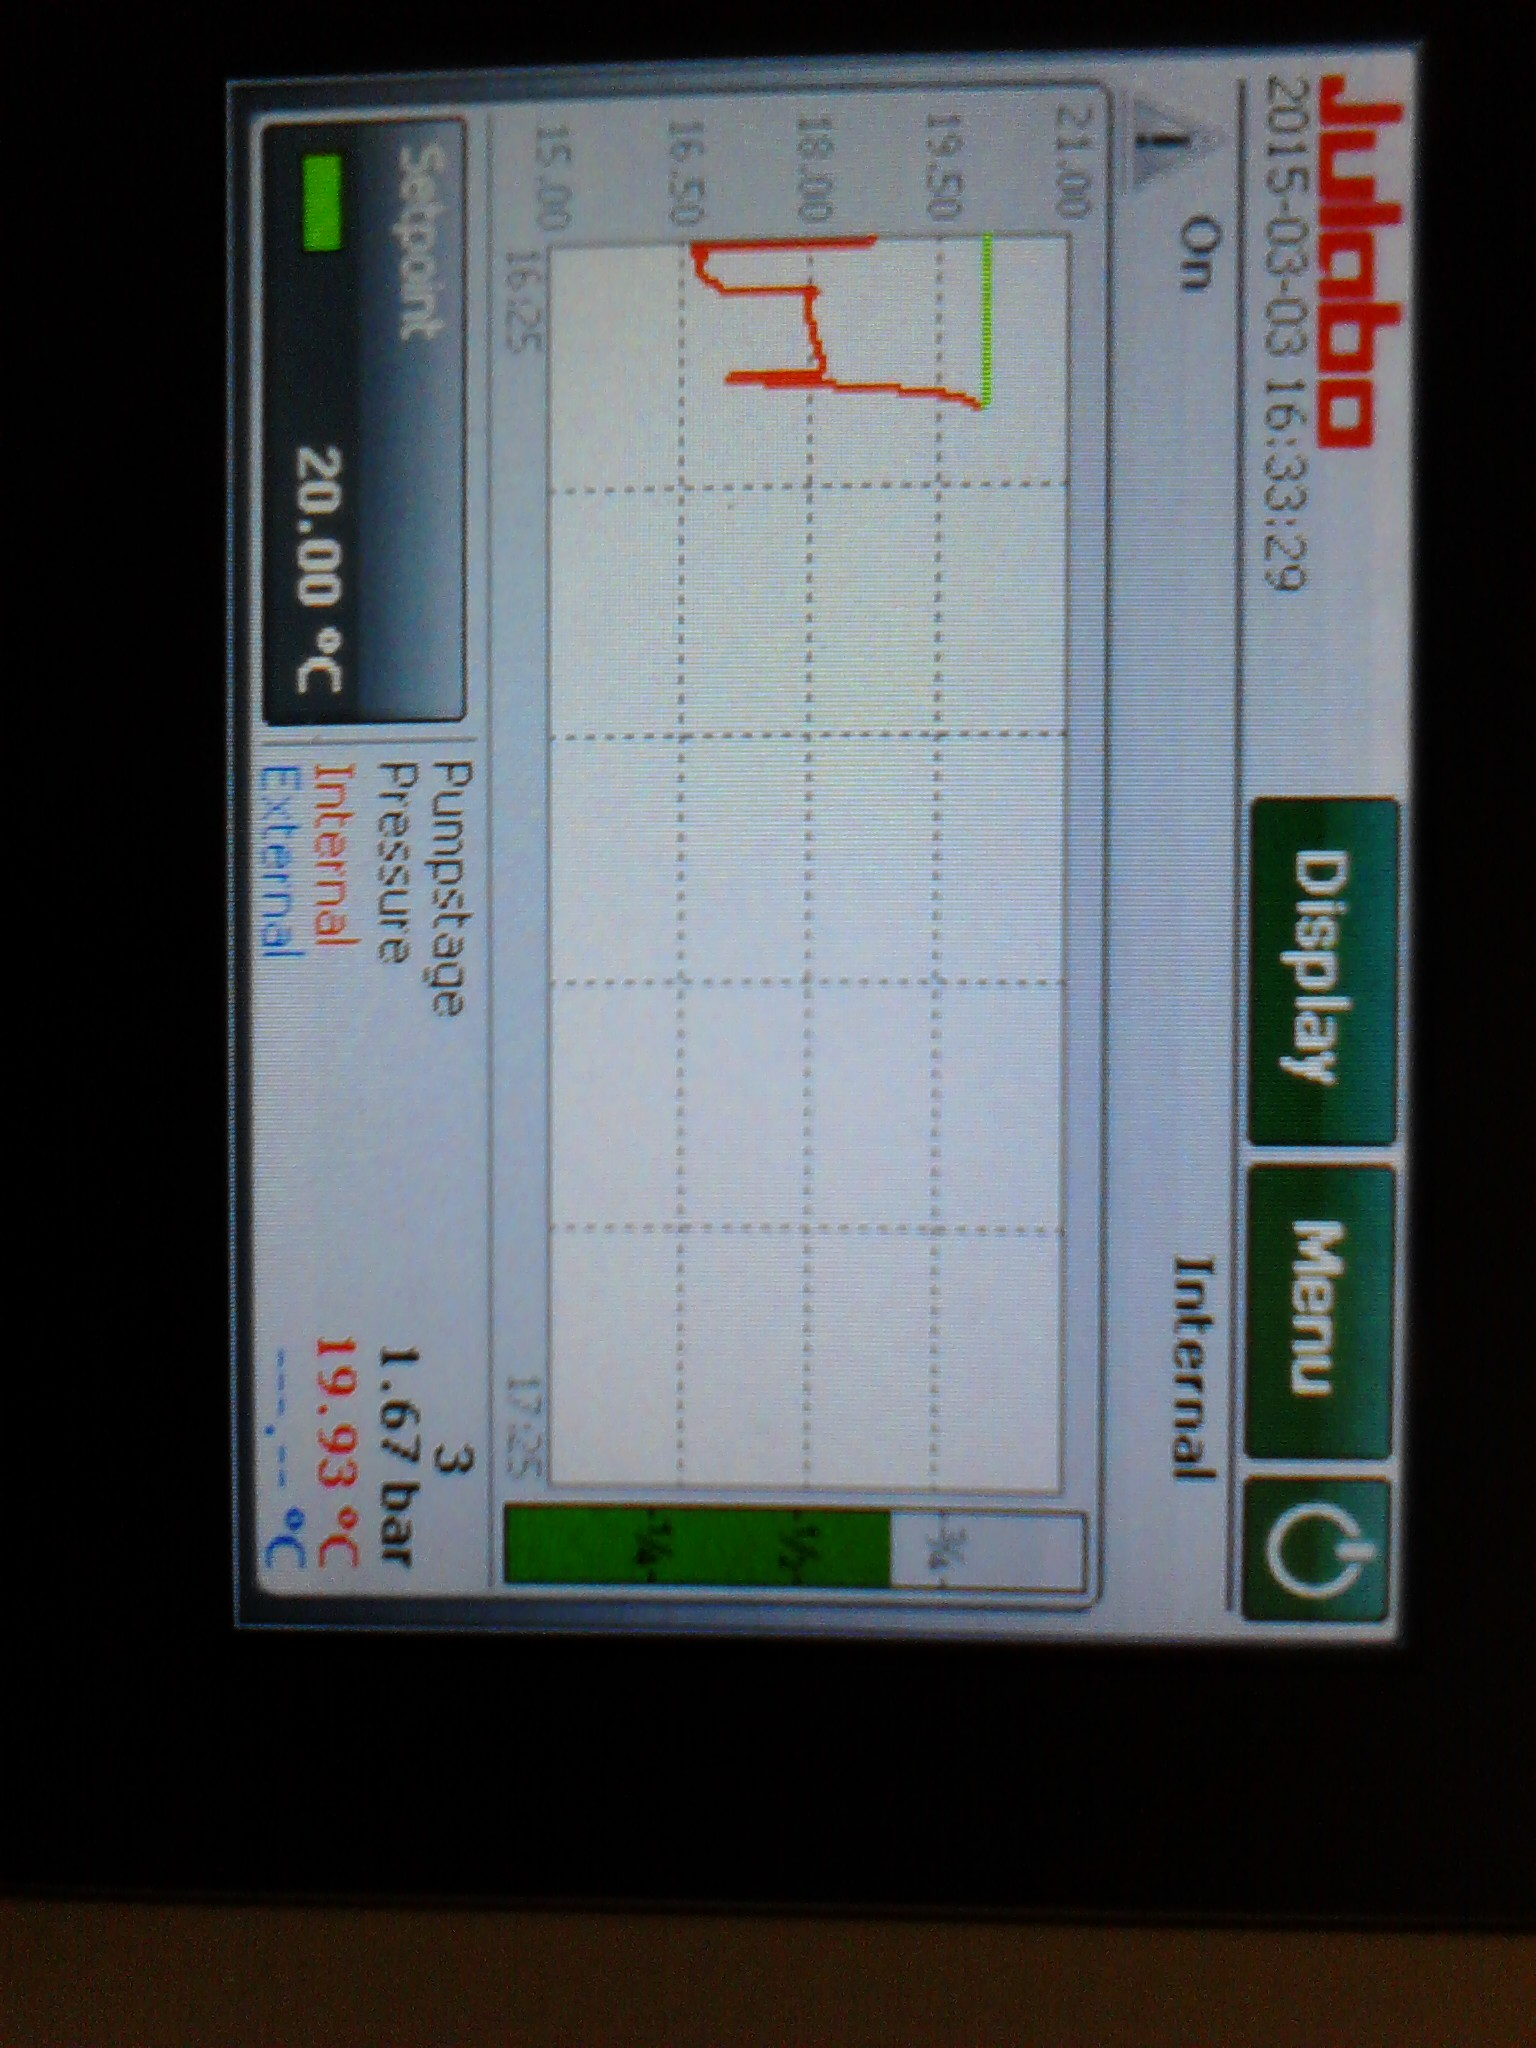
\includegraphics[angle=90,width=6cm]{figures/chiller_level6}
    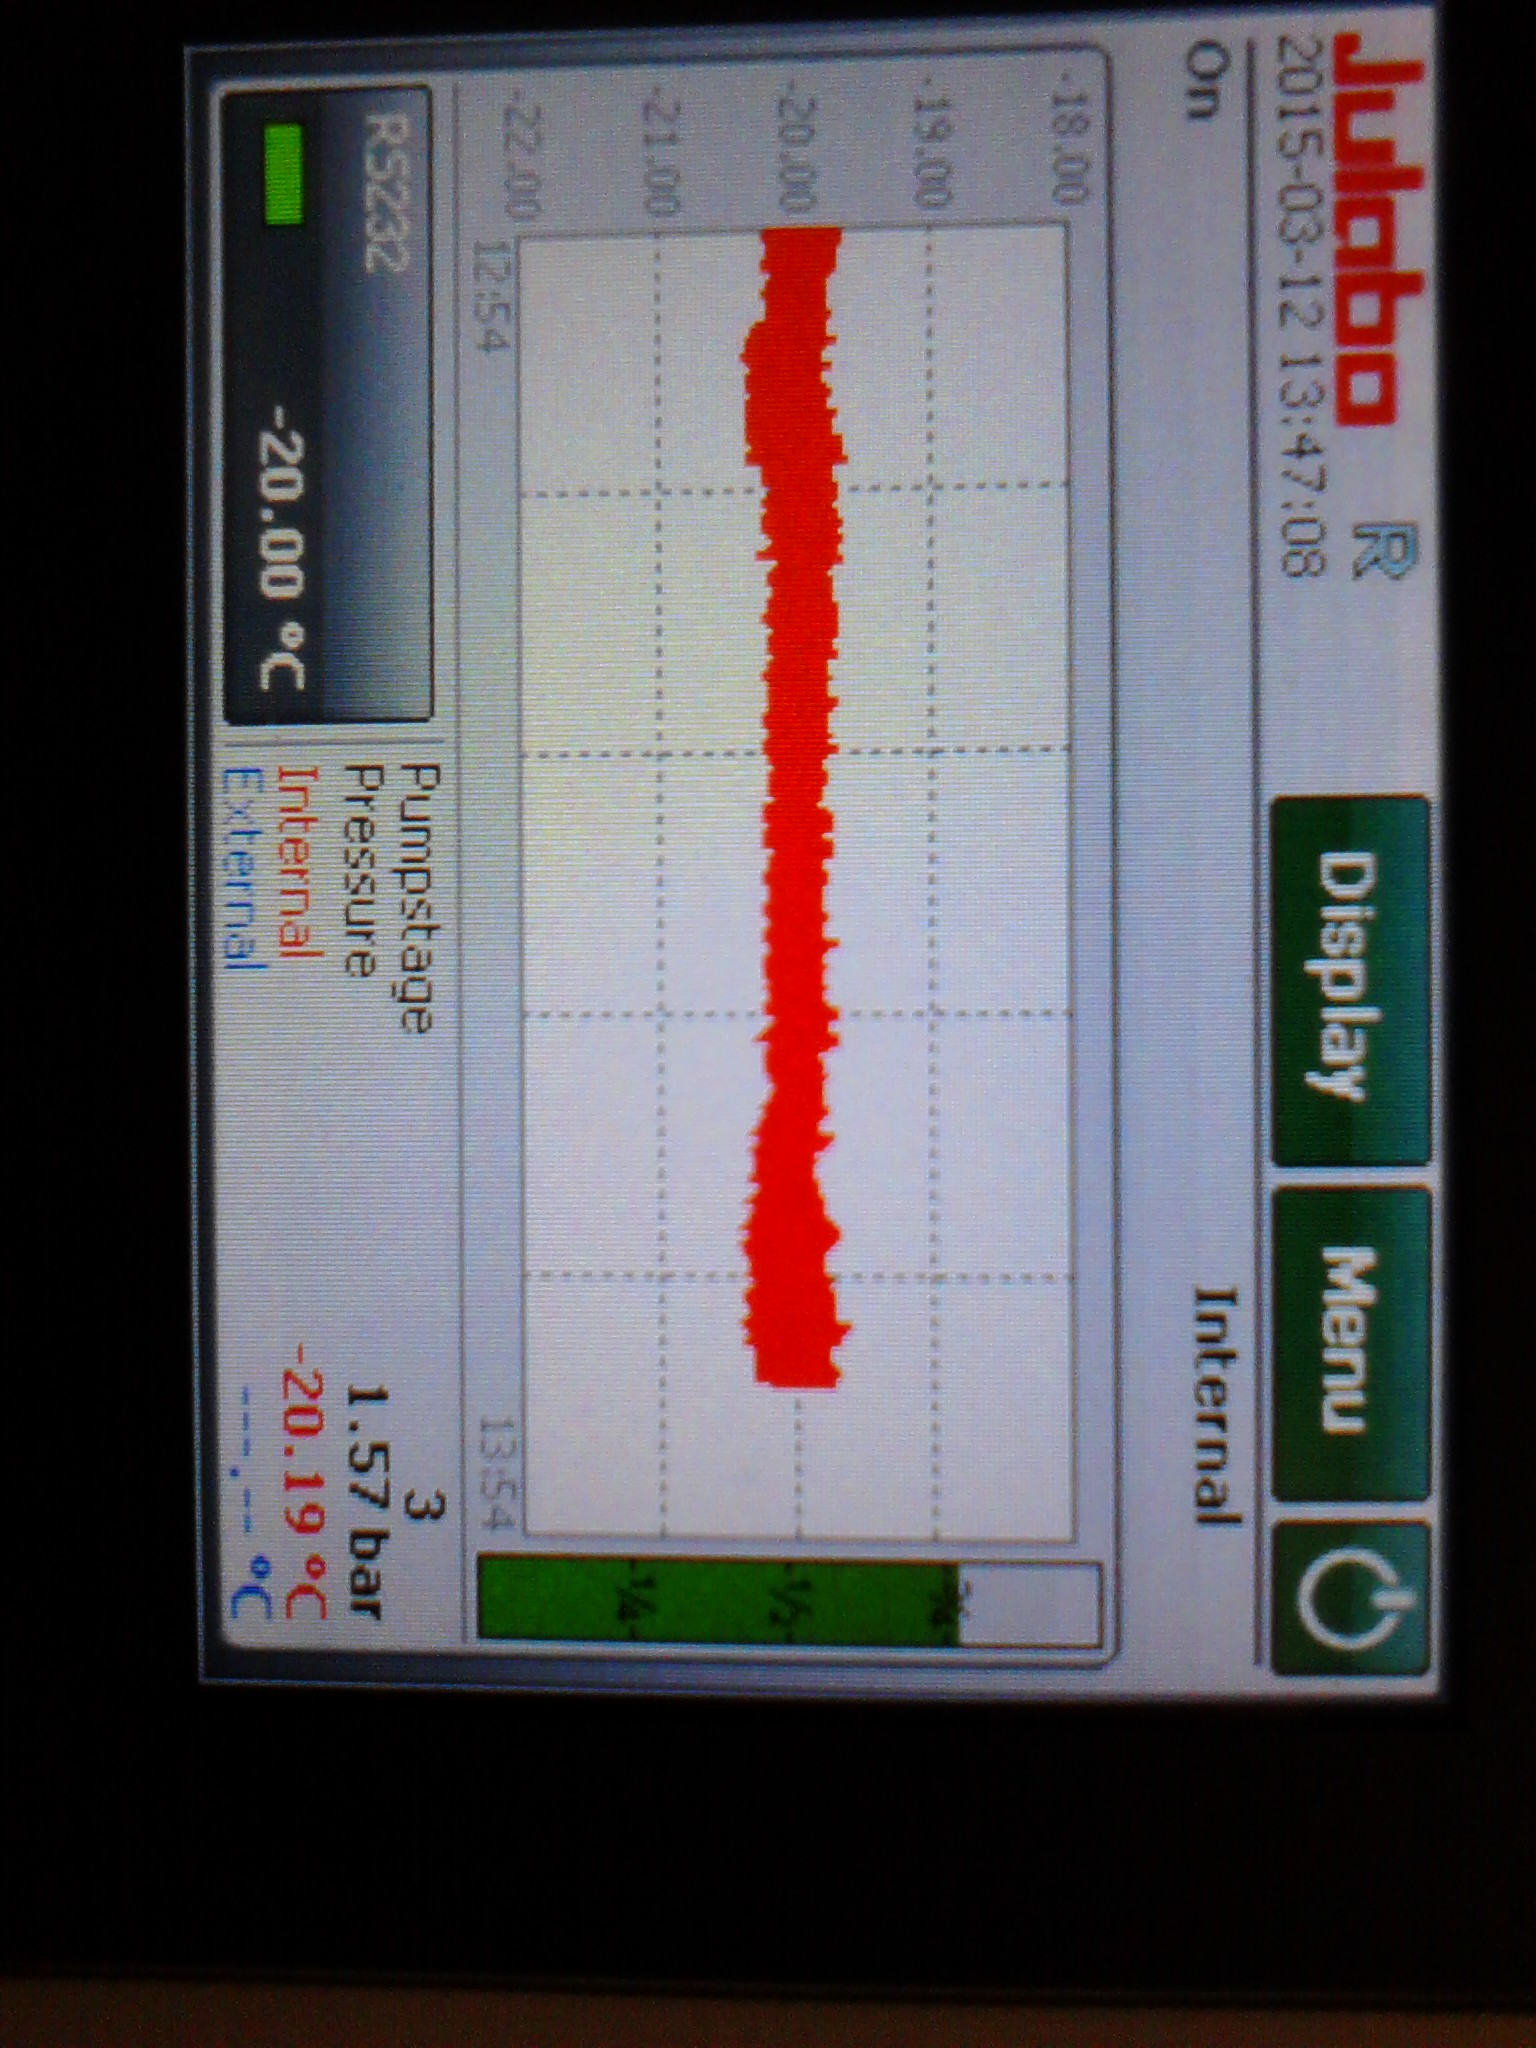
\includegraphics[angle=90,width=6cm]{figures/chiller_level7}
    \caption{Steps of the SVT chiller level indicator. Level 1 (first image) is the lowest level at which the chiller will continue to run, with a low level warning alarm. Levels 2--7 are levels for normal operation. Level 8 (not shown) will cause a high level warning alarm, but the chiller will continue to run. \label{fig:svt_chiller_level}}
\end{figure}

\subsection{Response to unexpected chiller trip}
\label{sec:proc_cooling_chillertrip}

\begin{enumerate}
    \item Look at the EPICS screens for the PLC. Check the alarm status fields for any PLC alarms. Also look at the software interlock screen and check the interlock status fields for any interlock faults. Call the SVT expert with the list of alarms.
    \item If the expert tells you to restart the chiller: Disable all PLC alarms that have tripped. Bypass and reset all software interlocks that have tripped. Start the chiller from its EPICS screen. As alarms clear, re-enable all alarms and interlocks that you disabled. If any alarm does not clear, call the SVT expert.
\end{enumerate}

